\documentclass[12pt,a4paper]{report}
\usepackage[Rejne]{fncychap}
\usepackage{titlesec}
\usepackage{biblatex}
\usepackage[utf8]{inputenc}
\usepackage[french]{babel}
\usepackage[T1]{fontenc}
\usepackage{amsmath}
\usepackage{amsfonts}
\usepackage{hyperref}
\usepackage{amssymb}
\usepackage{graphicx}
\usepackage{fullpage}
\usepackage{caption}
\usepackage{subcaption}
\usepackage[left=2cm,right=2cm,top=2cm,bottom=2cm]{geometry}
\usepackage{ragged2e}
\usepackage{listings}
\renewcommand\FmN[1]{}

\author{BERJOLA Matthias 37000961-ADOLPHE Benjamin 37001213}           %   



\begin{document}
\title{Projet Développement mobile: Planee}
\author{BERJOLA MATTHIAS 37000961 - ADOLPHE BENJAMIN 37001213}
\date{\today} 

\maketitle


\newpage

\tableofcontents
\newpage
\begin{abstract}
\begin{flushleft}
\justify
Android est un OS assez répandu de nos jours: Téléphones, tablettes, Tv etc.. De ce fait durant l'UE de développement mobile le choix de réalisé une application sous Android à été fait. Dans ce rapport sera détaillé le cheminement suivi  afin de coder l'application. On y trouve une description brève de l'application, une  architecture de celle-ci ainsi qu'une énumération des différents problèmes rencontrés.
\end{flushleft}
\end{abstract}
\chapter*{Introduction}  
\begin{flushleft}
\justify
Cette année, afin de valider l'UE développement mobile 2, nous avons dû réaliser un projet. Ce projet consistait à réaliser une application ou un jeu respectant certaines contraintes:
\begin{itemize}
\item[•] Le choix de l'application est laissé libre, mais une partie de la notation portera sur sa complexité (quelque chose de trop simpliste ne donnera pas lieu à beaucoup de points).
\item[•] L’application doit proposer : plusieurs écrans, une présentation
sous forme de liste, une sauvegarde persistante.
\item[•] L’application doit fonctionner correctement sur tout type d’écran (grand, petit…), en mode portrait et paysage : ressources alternatives sous Android + contraintes sur les composants graphiques.
\end{itemize}
De ce fait mon collègue et moi même avons opté pour une application. Après un BrainStorming intensif, nous avons décidé d'appeler notre application Planee et nous expliquerons son fonctionnement par la suite.
\end{flushleft}

\newpage
\chapter*{L'application Planee}
\section{Principe}
\begin{flushleft}
\justify
Planee est une application de gestion d'évènements. Elle permettra à l'utilisateur d'organiser et créer ses différents évènements. En effet, chaque évènement est composé d'un titre, d'une date limite de tâches et chaque tâche est composée d'un titre, d'un nom de magasin et éventuellement d'une URL indiquant le site du magasin si l'utilisateur a besoin de passer une commande. Sur le long terme l'application devrait supposer des magasins ou différents sites pour passer commande.
\end{flushleft}
\section{Architecture de l'application}
\begin{flushleft}
\justify
L'application Planee est structurée en 3 Activités:
\begin{itemize}
\item[•] L'activité MainActivity représente la page d'Accueil.
\item[•] L'activité AddActivity représente la page d'ajout d'un évènement.
\item[•] L'activité DetailActivity représente la page de détails d'un évènement.
\item[•] L'activité UpdateActivity représente la page de modification d'un évènement.
\end{itemize}
\end{flushleft}
\subsection{MainActivity}
\begin{flushleft}
\justify
Comme dit précédemment la MainActivity représente la page d'accueil. En effet, la MainActivity est composée principalement d'un élément ListView. La ListView permettra de lister les différents évènements. Les évènements sont récupérés dans la Base de Données locale du téléphone, si aucun évènement est présent dans la Base de Donnée alors un message apparaîtra à l'écran.\\

Quelques fonctionnalités de la page d'accueil:
\begin{itemize}
\item[•] Appuie long sur un évènement pour le supprimer
\item[•] Appuie sur un évènement pour avoir les détails suivants:
\begin{itemize}
\item[•] Nom de l'évènement
\item[•] Date de l'évènement
\item[•] Liste des taches de l'évènement
\end{itemize}
\item[•] Appuie sur le bouton retour pour quitter l'application
\end{itemize}
\begin{figure}[!h]
    \centering
    \begin{subfigure}[b]{0.3\textwidth}
        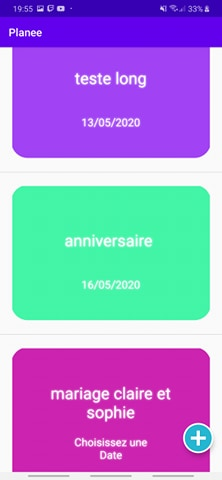
\includegraphics[width=\textwidth]{HomeWEvents1}
    \end{subfigure}
    \begin{subfigure}[b]{0.3\textwidth}
        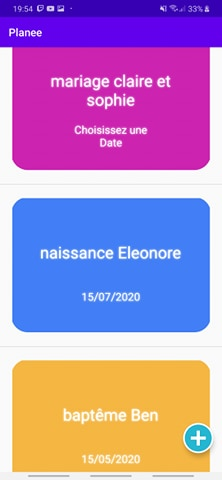
\includegraphics[width=\textwidth]{HomeWEvents2}
    \end{subfigure}
    \begin{subfigure}[b]{0.3\textwidth}
        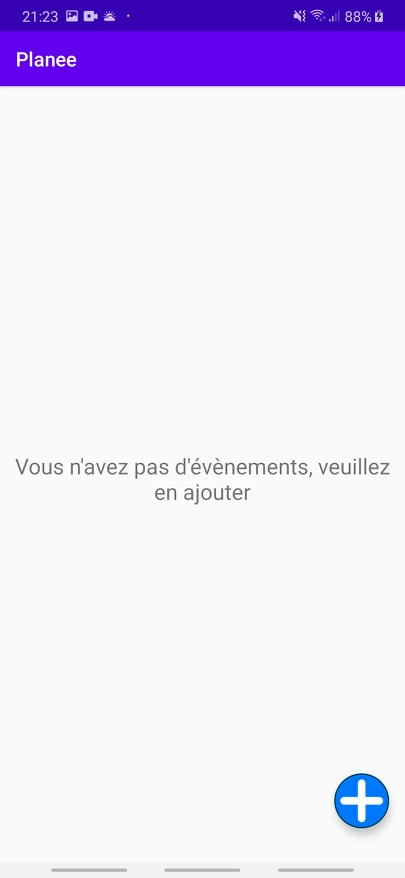
\includegraphics[width=\textwidth]{HomeNoEvent}
    \end{subfigure}
    \caption{Page d'accueil avec et sans évènements}
\end{figure}
\end{flushleft}
\subsection{AddActivity}
\begin{flushleft}
\justify
La page contient un formulaire permettant d'entrer le nom, la date limite de l'évènement, l'heure et l'ensemble des tâches. Le formulaire d'ajout de tâches est dynamique grâce au bouton "Nouvelle tâche".\\

Quelques fonctionnalités du formulaire:
\begin{itemize}
\item[•] Appuie sur le bouton "Nouvelle tâche" afin d'ajouter un champs de saisie d'une nouvelle tâches, ces champs sont composées de 3 champs de saisie de textes:
\begin{itemize}
\item[•] Nom de la tâche
\item[•] Potentiellement le nom du magasin
\item[•] Potentiellement l'URL du site du magasin
\end{itemize}
\item[•] Appuie sur le bouton "Ajout de l'évènement" afin d'ajouter l'évènement dans la base de données locale de l'appareil et déclencher une alarme à la date et l'heure entrées par l'utilisateur (Voir partie problèmes rencontrés)
\end{itemize}
\begin{figure}
    \centering
    \begin{subfigure}[b]{0.3\textwidth}
        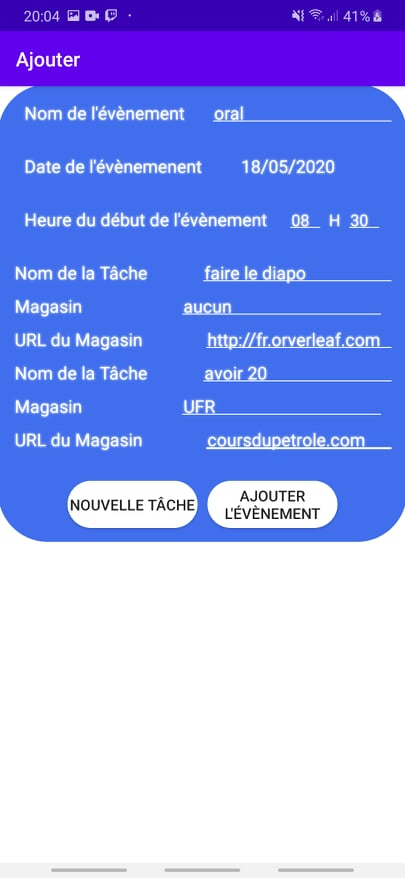
\includegraphics[width=\textwidth]{FormWTask}
    \end{subfigure}
    \begin{subfigure}[b]{0.3\textwidth}
        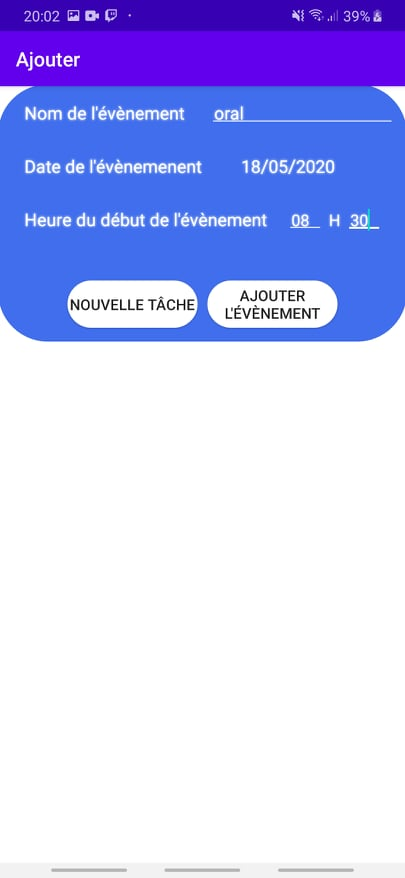
\includegraphics[width=\textwidth]{FormNoTask}
    \end{subfigure}
    \caption{Page du formulaire d'ajout avec et sans tâches}
\end{figure}
\end{flushleft}
\newpage
\subsection{DetailsActivty}
\begin{flushleft}
\justify
Comme dit dans la partie concernant la MainActivity, lors d'un appui sur un évènement on accède à la page de détails de cet évènement. Ainsi, on va récupérer tout les éléments dans la Base de données locale en rapport avec cet évènement.
Quelques fonctionnalités de la page:
\begin{itemize}
\item[•] Appuie sur une tache afin de la supprimer (Tache complétée)
\item[•] Appuie sur le bouton flottant afin de modifier l'évènement courant
\end{itemize}
\begin{figure}[!h]
    \centering
    \begin{subfigure}[b]{0.3\textwidth}
        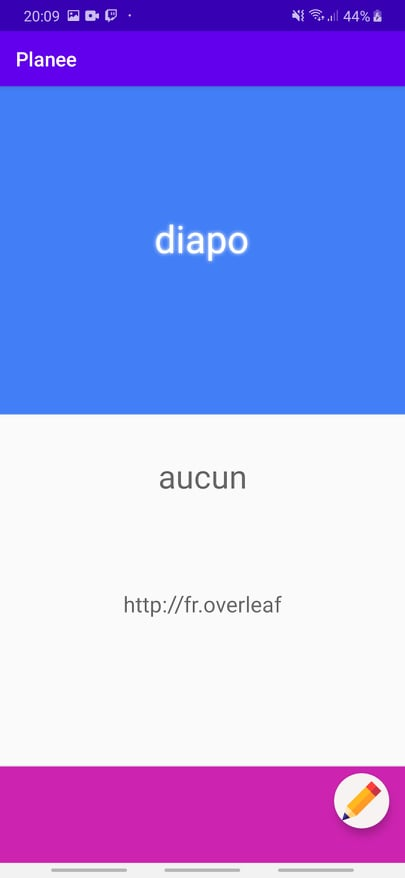
\includegraphics[width=\textwidth]{Tasks}
    \end{subfigure}
    \begin{subfigure}[b]{0.3\textwidth}
        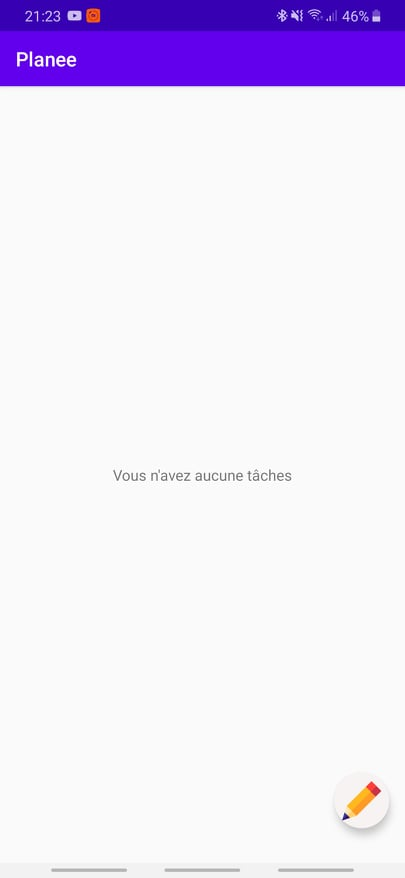
\includegraphics[width=\textwidth]{NoTask}
    \end{subfigure}
    \caption{Formulaire de mise à jour avec et sans modification(s)}
\end{figure}
\end{flushleft}
\newpage
\subsection{UpdateActivity}
\begin{flushleft}
\justify
Le layout présent dans UpdateActivity est le même que celui présent dans AddActivity. En effet, la seule différence entre ces deux activités est que l'un est fait pour mettre à jour un évènement l'autre pour ajouter. Ainsi, le formulaire de mise à jour sera pré-remplis par les informations de l'évènement voulu par l'utilisateur. \`A partir de ce formulaire, l'utilisateur pourra mettre à jour les données existantes mais aussi ajouter de nouvelles tâches. 
\begin{figure}[!h]
    \centering
    \begin{subfigure}[b]{0.3\textwidth}
        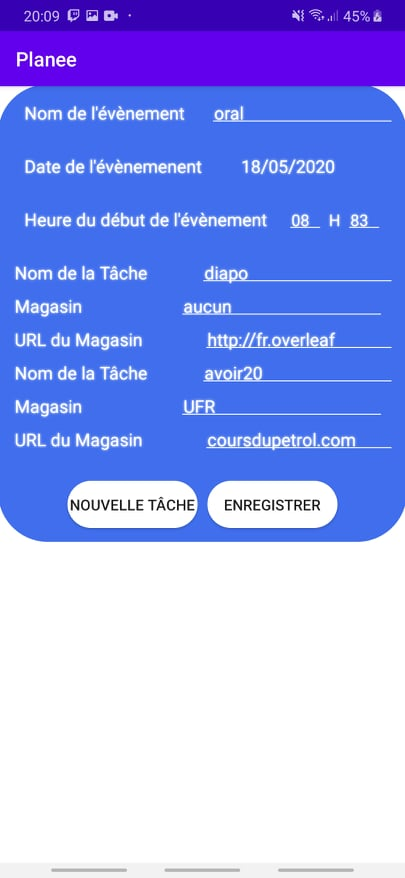
\includegraphics[width=\textwidth]{FormUpdateNoModif}
    \end{subfigure}
    \begin{subfigure}[b]{0.3\textwidth}
        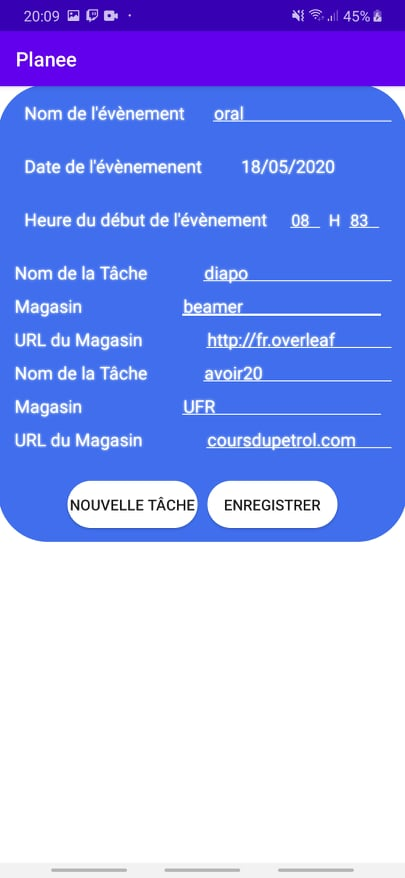
\includegraphics[width=\textwidth]{FormUpdateModif}
    \end{subfigure}
    \begin{subfigure}[b]{0.3\textwidth}
        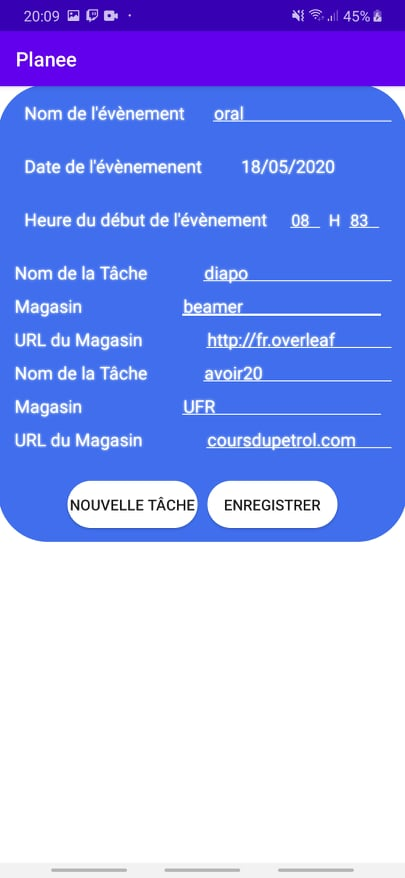
\includegraphics[width=\textwidth]{FormUpdateModif}
    \end{subfigure}
    \caption{Formulaire de mise à jour avec et sans modification(s)}
\end{figure}
\end{flushleft}
\newpage
\subsection{Bases de données}
\begin{flushleft}
\justify
Pour ce projet, nous avons utilisé une base de données composée de 2 tables:
\begin{itemize}
\item[•] Une table Event\_Table
\item[•] Une table Tache\_Table
\end{itemize}
\medskip
La table Event\_Table sert à stocker les différents évènements créé. À l'intérieur on y trouve :
\begin{itemize}
\item[•] l'id de l'évènement
\item[•] Le nom de l'évènement
\item[•] Sa date limite(La date où l'évènement se produira)
\item[•] L'heure limite (L'heure à laquelle l'évènement se déroulera)
\end{itemize}
\medskip 
La table Tache\_Table sert quand à elle à stocker les différentes tâches à stocker les différentes tâches à effectuer afin de préparer l'évènement convenablement. Elle est composée de:
\begin{itemize}
\item[•] L' id de la tâche
\item[•] Du nom du magasin dans lequel la tâche doit être effectué
\item[•] De l'URL du magasin si l'achat peut être effectuer en ligne
\item[•] IdEvent qui est une clé étrangère permettant de savoir à quel évènement appartient la tâche
\end{itemize}
\medskip 
On trouve également deux méthodes indispensables à la base de données :
\begin{itemize}
\item[•] La méthode InsertEvent
\item[•] La méthode getAllEvent
\end{itemize}
\medskip 
La première méthode a été crée dans le but de pouvoir insérer chaque événements(composé de tâches) dans la base de données. La seconde méthode permet de récupérer tout les évènements crées par l'utilisateur afin de pouvoir les afficher de nouveau lorsque l'utilisateur reviens sur l'application après l'avoir fermé. \\
Le choix d'une base données a été fait dans le but de garantir la persistance des données de l'utilisateur à chaque fois que l'application est quittée puis ré-ouverte.

\begin{figure}[!h]
    \centering
    \begin{subfigure}[b]{0.3\textwidth}
        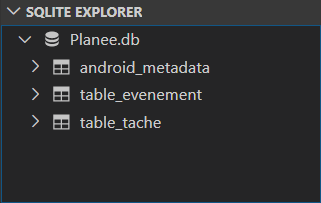
\includegraphics[width=\textwidth]{SchemaBDD}
    \end{subfigure}
    \begin{subfigure}[b]{0.3\textwidth}
        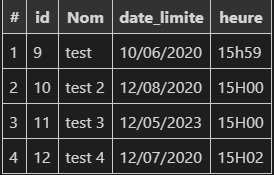
\includegraphics[width=\textwidth]{TableEvent}
    \end{subfigure}
    \begin{subfigure}[b]{0.3\textwidth}
        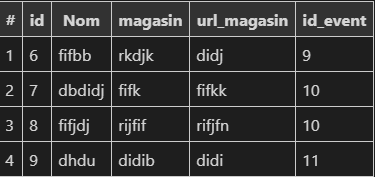
\includegraphics[width=\textwidth]{TableTache}
    \end{subfigure}
    \caption{Schéma de la Base de données}
\end{figure}
\end{flushleft}
\section{Problèmes rencontrés}
\begin{flushleft}
\justify
Au cours de ce projet, nous avons rencontré plusieurs problèmes. Nous allons donc citer dans ce rapports les différents problèmes que nous avons rencontré.
\end{flushleft}
\subsection{Fragments}
\begin{flushleft}
\justify
Au début de ce projet, lors du choix de la première activité, nous avons choisi l'activité "Navigation Drawer Activity".\cite{1}\\
\center
\begin{minipage}{0.48\linewidth}
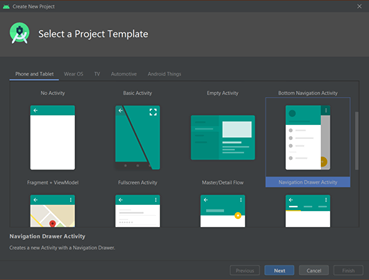
\includegraphics[width=\linewidth]{Template}
\captionof{figure}{Template}
\end{minipage}
\justify
Cependant, ce template est basé sur l'utilisation des 
Fragments, une notion qui n'a pas été vue en cours. Ainsi nous avons suivi de nombreux tutoriaux concernant les Fragments. Voici une liste des différents problèmes rencontrés lors de l'utilisation de Fragment: 
\begin{itemize}
\item Dès lors que l'on a voulu changer de page, le premier problème est apparu. En effet, lors de l'utilisation du FragmentManager et des transitions afin de changer les Fragments ils avaient tendance à se superposer. 
\center
\begin{minipage}{0.48\linewidth}
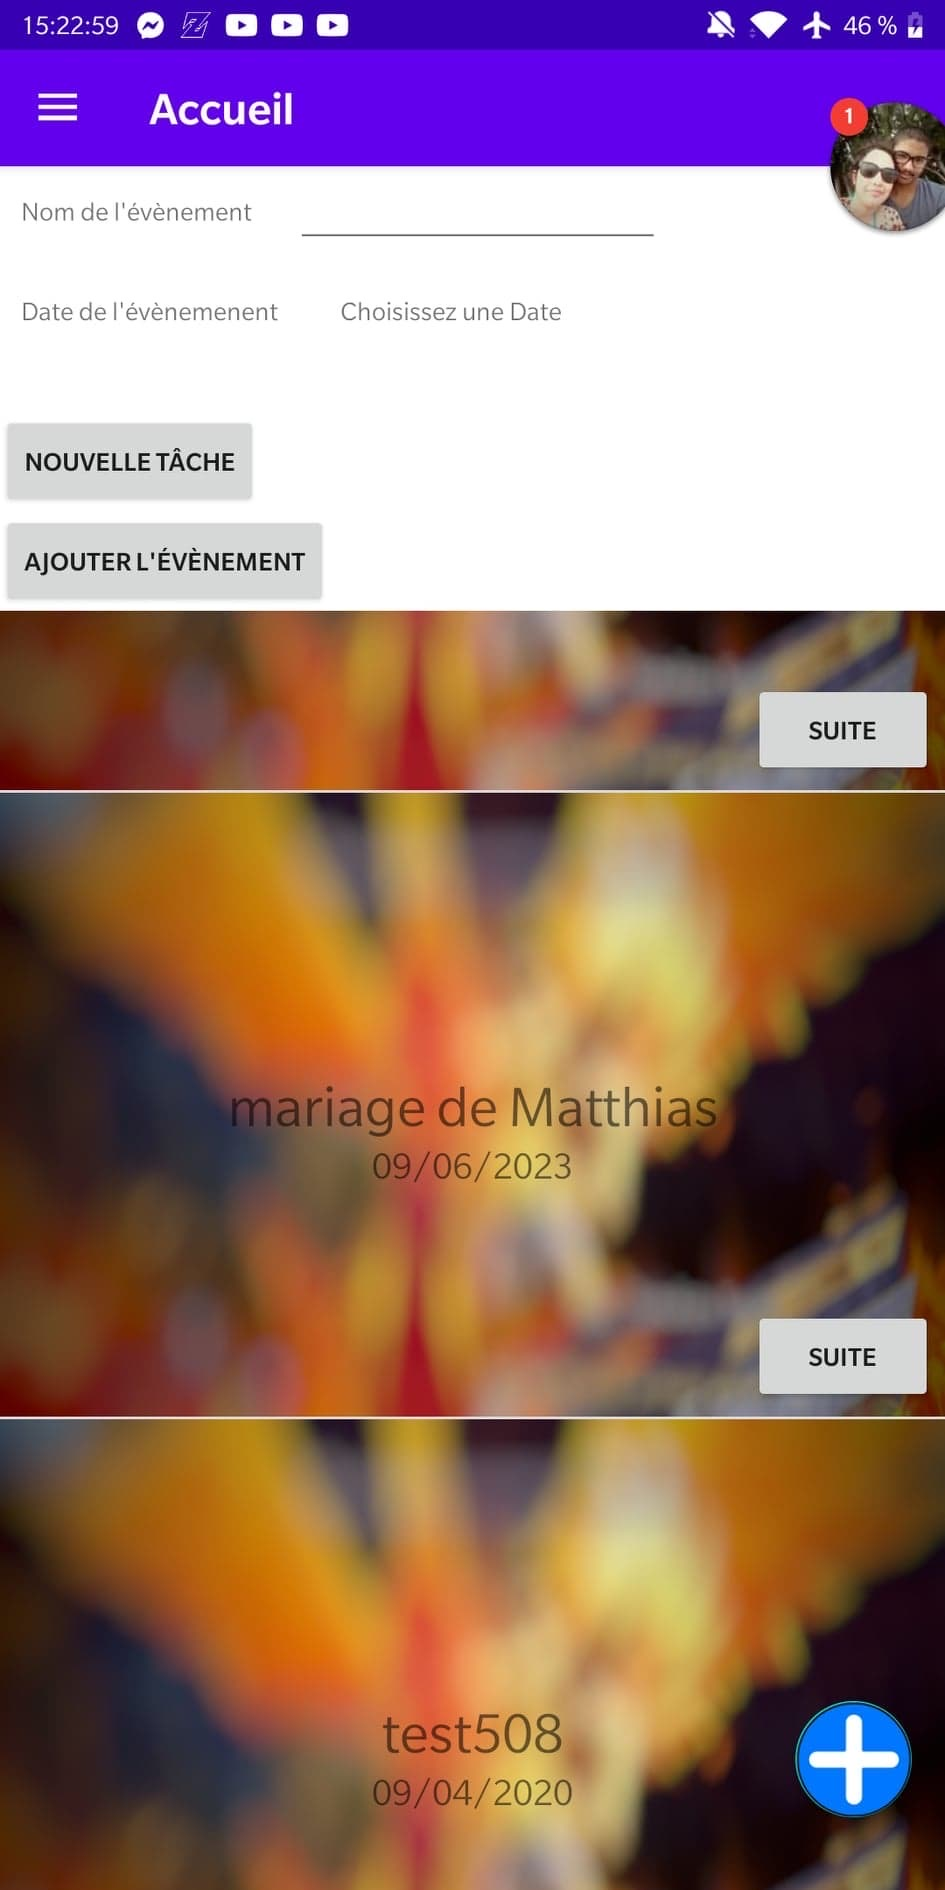
\includegraphics[width=\linewidth]{SupperPosFrag}
\captionof{figure}{Template}
\end{minipage}
\justify
\item Nous avons pu résoudre ce problème en vérifiant dans le conteneur si un fragment était présent et si c'était le cas on enlevait tout fragment du conteneur grâce au code suivant:
\end{itemize}
\begin{lstlisting}
	if (container != null) {
		container.removeAllViews();
	}
\end{lstlisting}
\begin{itemize}
\item Nous devions gérer l'appuie sur le bouton retour de l'utilisateur. En effet, lorsque l'utilisateur appuyait sur la touche retour il se retrouvait devant une interface blanche car nous vidions le conteneur à chaque fois. Ainsi dans chaque fragment nous avons du gérer de façon programmative l'appui sur le bouton retour sachant que la méthode "OnBackpressed" ne fonctionnait pas dans le cas de Fragments:
\end{itemize}
\begin{lstlisting}
	// This callback will only be called when 
	MyFragment is at least Started.
        OnBackPressedCallback callback = 
        new OnBackPressedCallback(true /* enabled by default */) {
            @Override
            public void handleOnBackPressed() {
                getFragmentManager().beginTransaction()
                .replace(R.id.DetailsFragment, new HomeFragment())
                .addToBackStack(null)
                .commit();
            }
        };
        requireActivity().getOnBackPressedDispatcher()
        .addCallback(this, callback);
\end{lstlisting}
\begin{itemize}
\item Le problème le plus important que nous avons rencontré était le temps. En effet, se former sur les Fragments et tout ce qui touchait aux Fragments demandaient énormément de temps. Plus de temps nous passions à nous former moins de temps nous avions pour terminer l'application. Ainsi après 3 séances supplémentaires avec le responsable de cet UE et de nombreuse galères dans la programmation avec les Fragments, nous avons décidé de repasser dans un format classique en privilégiant les activités aux Fragments malgré l'économie d'énergie apporté par les Fragments en utilisant qu'une seule activité pour tout gérer.
\end{itemize}
\end{flushleft}
\subsection{Notifications}
\begin{flushleft}
Lors de la réalisation du code concernant l'envoie de notifications de l'application afin de prévenir l'utilisateur le jour d'un évènement. Ainsi, pour créer la notification nous sommes passé par le code suivant:
\center
\begin{minipage}{0.8\linewidth}
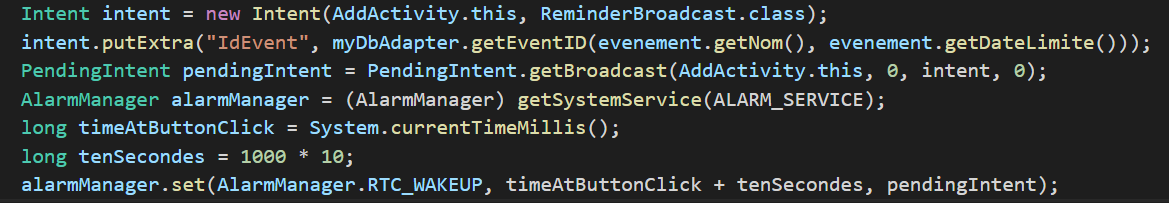
\includegraphics[width=\linewidth]{AlarmSet}
\captionof{figure}{Code de mise en place de l'alarme}
\end{minipage}
\justify
Le but de ce code est de créer une alarme pour la date de l'évènement afin d'envoyer une notification à l'utilisateur lorsque l'utilisateur ajoute un évènement à la base de données. Pour la création de cette notification, nous avons utilisé le code suivant: 
\center
\begin{minipage}{0.8\linewidth}
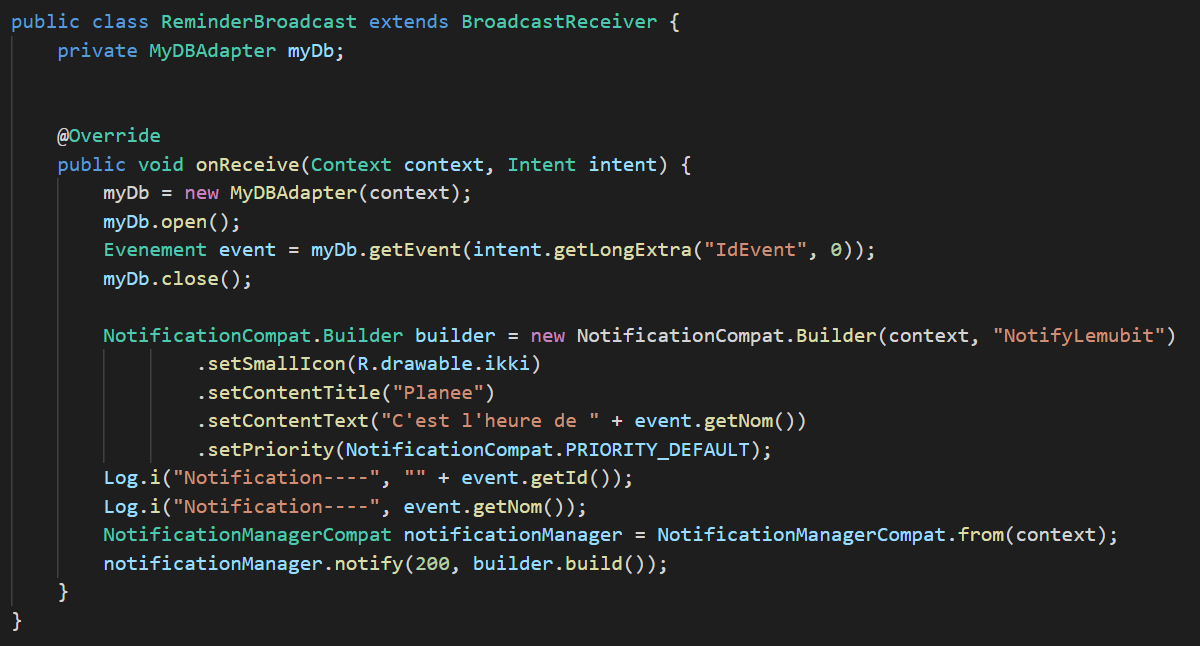
\includegraphics[width=\linewidth]{NotifCode}
\captionof{figure}{Code de mise en place de la notification}
\end{minipage}
\justify
Pour créer la notification, nous récupérons l'évènement récemment créé grâce à la méthode getEvent de MyDbAdapter et ensuite créer la notification à l'aide du Notification.Builder et du NotificationManagerCompat. Cependant, nous avons rencontré un problème qui, aujourd'hui, n'est toujours pas résolu. Pour les tests nous avons créer l'alarme pour un déclenchement dans 10 secondes. Lors de la création de 2 évènements, le texte de la notification en se met pas à jour. La notification conserve les éléments de la 1\up{ère} notification. Quelques fois, les informations sont null.
\begin{figure}[!h]
    \centering
    \begin{subfigure}[b]{0.3\textwidth}
        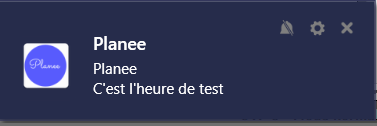
\includegraphics[width=\textwidth]{Notif}
    \end{subfigure}
    \begin{subfigure}[b]{0.3\textwidth}
        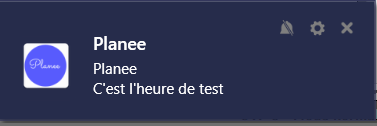
\includegraphics[width=\textwidth]{Notif}
    \end{subfigure}
    \caption{Problème : Notifications sur 2 évènements}
\end{figure}
\justify
Un autre problème s'est également révélé lors des tests de notification sur Android Studio. En effet selon la version d'Android utilisé, il fallait créer un "channel" manuellement sur lequel la notification serait diffusé. Le message d'erreur suivant s'affichait alors dans le logCat:
\\

\begin{minipage}{\linewidth}
\centering
\includegraphics[scale=0.3]{logCatNotif}
\captionof{figure}{Message d'erreur LogCat}
\end{minipage}\\
Bien évidemment c'est en épluchant le net qu'une réponse nous a été apporté sur le site StackOverflow\cite{2}
\end{flushleft}
\subsection{Layout}
\begin{flushleft}
\justify
Lors de la réalisation du design de l'application nous devions géré en plus des éléments de bases(couleurs formes etc) les layouts. Deux problèmes revenais souvent: La conservation de l'échelle lorsque l'on passe à un appareil plus petit et la superposition des éléments lors de ce passage.\\
Au départ le design de l'application était réalisé entièrement avec des ConstraintLayout. Le problème avec les Constraint Layout est le manque de précision et de rigidité dans les contraintes que nous mettons. De ce fait des éléments qui semblait bien placés se retrouvait déplacés sans aucune intervention de notre part lorsque nous lançons l'application. Nous avons donc pris la décision de remplacer les Constraint Layout par des Relative Layout là où cela posait problème(page détail, page addDétail notamment). Après ce changement nous avons pu convenablement placé les différents éléments sans erreurs apparentes.
\end{flushleft}
\section{Amélioration futures}
Bien que l'application soit fonctionnelle, il y a des améliorations possibles afin de rendre l'application plus attractive, beaucoup plus fonctionnelle mais aussi plus proche de ce à quoi ressemble les applications de nos jours.
Parmis ces améliorations on pense notamment à:
\begin{itemize}
\item[•]Un système de notification fonctionnelle 
\item[•]un système  de connexion afin de pouvoir stocker des informations dans le cloud 
\item[•]Adaption de l'application sur écran plus large, plus récent( 18:9 etc...)
\item[•]Mise en place de l'application sur IOS 
\item[•]Design plus épuré et plus actuel/professionnel 
\end{itemize}

 
\newpage
\chapter*{Conclusion}
\begin{flushleft}
\justify
En conclusion,  nous pouvons dire que nous avons atteint l'objectif que nous nous étions fixé : Créer une application sous Android qui comporte plusieurs écrans, une présentation sous forme de liste et qui garantit une persistance des données de l'utilisateur. Il y a certes encore des améliorations à apporté à l'application afin qu'elle soit "conforme" à ce qu'il se trouve actuellement sur le marché mais le résultat sur le plan technique est déjà plus que satisfaisant.Nous avons également appris à faire l'impasse sur certaines solutions trop compliquées à mettre en place dans le temps imparti et à en favoriser d'autres qui produisent le même résultat, certes pas tout à fait similaire à celui attendu initialement mais qui remplit quand même la fonction attendu.Ce projet nous a également permis d'asseoir nos compétences en matière de communication mais surtout du partage et suivi de travail via l'utilisation de la plateforme Github\cite{3}.
\end{flushleft}
\newpage
\begin{thebibliography}{2} 
   \bibitem[1]{Android} \href{www.android.developper.com}{AndroidDevelopper}, 2019, 
   \bibitem[2]{Stack} Md Imran Choudhury, Janvier 2020, \href{https://stackoverflow.com/a/16448278}{Réponse StackOverflow}
    \bibitem[3]{github} \href{www.github.com}{Github}, 2020
    
\end{thebibliography} 
\end{document}
